\subsection{E4: structure (exploratory)}
\label{sec:e4}

When a corridor in the LU cut is blocked, the reservation-impact-set share of funnel and high fluctuates across random seeds (Table~\ref{tab:e4}).
In direction, funnel is higher (median \(0.254\) vs.\ \(0.204\); mean \(0.244\) vs.\ \(0.229\)),
but \emph{the two groups overlap heavily}: funnel lies in \([0.180,0.309]\) and high in
\([0.156,0.372]\), so the latter interval fully contains the former, and a single random seed suffices to reverse the direction
(on random seed \(2024\), high reaches \(0.372\), above funnel's \(0.296\)).
With five random seeds and two layouts, this gap supports no conclusion.
Under the busy-corridor blockage protocol of Section~\ref{sec:e1}, the three equal-size layouts also yield
\(\mathrm{Cl}/|R|\) within the narrow band \EoneCloLo--\EoneCloHi, and again fail to separate the layouts.

\textbf{External layouts are used to separate the causes of the negative result.}
The three equal-size layouts all belong to the dumbbell family and differ little in geometry (Table~\ref{tab:e4pub}: \(9\)--\(11\) nodes,
\(8\)--\(12\) corridors, and an LU cut of only \(1\) or \(2\)). On these layouts, two explanations cannot be told apart: ``the metric is too coarse''
and ``the instances differ too little in geometry''. The second batch of instances in Section~\ref{sec:protocol}
serves to separate the two (Table~\ref{tab:e4pub}).

\textbf{The results on the external layouts run opposite to the expected direction.}
This batch contains only \NPubNets\ independent samples of network geometry (Section~\ref{sec:protocol}), so we use it only to examine the machine-configuration dimension.
On \emph{the same} \(4\times 4\) network, changing only the number and placement of machines from \(4\) to \(5\)
drops the median impact-set share from \PubCloHi\ to \PubCloLo, a range of \PubCloSpread.
On the same \(5\times 5\) network, three machine configurations (\(6\), \(7\), and \(8\) machines) give a range of \PubCloSpreadBig.
For comparison, the three in-house layouts, which are \emph{matched parameter by parameter} but use three \emph{different} networks,
give shares only within \SelfCloLo--\SelfCloHi, a range of \SelfCloSpread.
Thus, \textbf{with the network fixed and the machine configuration varied, the impact-set share can vary more than it does across three different networks}:
about four times as much on the \(4\times 4\) network and about one and a half times as much on the \(5\times 5\) network.
The comparison is not symmetric. The external side changes both the number and the placement of machines, whereas the in-house side changes only the network; moreover, the three in-house layouts differ little in geometry,
so \SelfCloSpread\ is only a \emph{lower bound} on the effect of ``changing the network''. The comparison therefore shows that the machine-configuration dimension cannot be ignored,
but not that its effect exceeds that of network geometry.

\textbf{A minimum cut determined by the network alone cannot explain the size of the impact set.}
On these \NPubInst\ external instances, \textbf{the LU cut is always \(2\) and the funnel share is always \(0\)}.
Both networks place the load/unload stations at grid corners, and a corner of a four-neighbor grid has exactly two outgoing edges, so the cut value is fixed at \(2\).
The other layout family shipped with the same toolkit (excluded from this batch because it allows diagonal moves) places the load/unload stations at edge midpoints of the grid, where the out-degree is \(3\).
\textbf{On real layouts, this metric therefore takes only a few discrete values determined by the grid positions of the load/unload stations}, rather than varying continuously with geometry.
More importantly, \textbf{both metrics stay constant across all the above variations}, while the quantity to be explained varies by
\PubCloSpread; a metric with a constant value cannot explain a varying quantity. The third metric (corridors per node) takes only two values over the whole batch (\(23/16\) and
\(38/25\)), which is likewise insufficient to explain the within-group variation.

Hence, \textbf{on these \NPubInst\ external instances and the three in-house layouts, static cuts do not explain the size of the impact set}.
This family of metrics was designed for the tunable exit bottleneck at the load/unload stations of dumbbell layouts; on real layouts it degenerates into constants and has no explanatory power.
The alternative direction thus points to the demand side: the size of the impact set may be determined not by how many paths the network \emph{can} provide, but by
\emph{the spatial distribution of demand}; concrete candidate quantities are given in Section~\ref{sec:future}.
This subsection reports an exploratory negative result and corresponds to none of the contributions.

\begin{table}[t]
\centering
\caption{E4 reservation-impact-set share \(\mathrm{Cl}/|R|\) (blocking a corridor in the LU cut; random seeds \(42,7,2024,99,123\)).
The instances in this table have \(12\) jobs / \(8\) machines / \(12\) vehicles, with the transport-to-processing time ratio calibrated to \(4.0\).
\textbf{This setting differs from that of Table~\ref{tab:e4pub}} (\(8\) jobs / \(4\) machines / \(4\) vehicles,
ratio \(1.0\), ten random seeds). Although both tables use the layout names \texttt{funnel}/\texttt{high},
\emph{values are not comparable across the two tables}; only the rows within Table~\ref{tab:e4pub} form a like-for-like comparison.}
\label{tab:e4}
\small
\begin{tabular}{@{}lcccccc@{}}
\toprule
Layout & \(42\) & \(7\) & \(2024\) & \(99\) & \(123\) & Median \\
\midrule
funnel & \(0.254\) & \(0.181\) & \(0.296\) & \(0.309\) & \(0.180\) & \(0.254\) \\
high & \(0.156\) & \(0.204\) & \(0.372\) & \(0.229\) & \(0.184\) & \(0.204\) \\
\bottomrule
\end{tabular}
\end{table}

\begin{table}[t]
\centering
\caption{E4 comparison of in-house and external layouts (blocking a corridor in the LU cut, ten random seeds; median \(\mathrm{Cl}/|R|\)).
All rows are matched parameter by parameter and differ only in network and machine configuration. \textbf{The external instances lie on only \NPubNets\ networks}
(\(\mathrm{N}_1\): \(4\times 4\) with one edge removed; \(\mathrm{N}_2\): \(5\times 5\) with two edges removed).
Rows within a group \emph{share the same network} and differ only in the number and placement of machines. The ``range'' column is given \emph{within each group};
the \(\mathrm{N}_1\) group has only \(2\) rows and the in-house group \(3\) rows, so ratios of ranges across groups indicate only the order of magnitude.
The LU cut and the funnel share are \emph{constant} over the entire external batch.}
\label{tab:e4pub}
\small
\begin{tabular}{@{}llcccccc@{}}
\toprule
\makecell{Source/\\network} & Instance & Machines & \makecell{Nodes/\\corridors} & LU cut & \makecell{Funnel\\share} & \(\mathrm{Cl}/|R|\)
 & \makecell{Within-group\\range} \\
\midrule
External \(\mathrm{N}_1\) & \texttt{LyuL2} & \(4\) & \(16/23\) & \(2\) & \(0\) & \(0.512\) & \\
External \(\mathrm{N}_1\) & \texttt{LyuL3} & \(5\) & \(16/23\) & \(2\) & \(0\) & \(0.305\)
  & \(\PubCloSpread\) \\
\cmidrule{1-8}
External \(\mathrm{N}_2\) & \texttt{LyuL4} & \(6\) & \(25/38\) & \(2\) & \(0\) & \(0.385\) & \\
External \(\mathrm{N}_2\) & \texttt{LyuL5} & \(7\) & \(25/38\) & \(2\) & \(0\) & \(0.422\) & \\
External \(\mathrm{N}_2\) & \texttt{LyuL6} & \(8\) & \(25/38\) & \(2\) & \(0\) & \(0.460\)
  & \(\PubCloSpreadBig\) \\
\midrule
In-house & \texttt{high} & \(4\) & \(10/10\) & \(2\) & \(0.286\) & \(0.497\) & \\
In-house & \texttt{funnel} & \(4\) & \(9/8\) & \(1\) & \(0.286\) & \(0.491\) & \\
In-house & \texttt{mid} & \(4\) & \(11/12\) & \(2\) & \(0.286\) & \(0.446\)
  & \(\SelfCloSpread\) \\
\bottomrule
\end{tabular}
\end{table}

\subsection{E5: trade-off against global rescheduling}
\label{sec:e5}

This subsection tests whether a \emph{crossover} exists, that is, whether bounded repair dominates under tight budgets while warm-started global rescheduling
overtakes it in \(C_{\max}\) once the budget is relaxed. \textbf{No such crossover exists within the tested range of \(0.2\)--\(2\)\,s,
and the conclusion extrapolates to larger budgets}. This follows from the shapes of the two curves. R2 is a single deterministic computation:
the three budget levels of a cell share the same computation, so \(C_{\max}\) does not vary with the budget. R0+ reports the best-so-far value per generation;
with the random seed fixed, a larger budget only lets the same search trajectory run for more generations, so \(C_{\max}\) is monotonically non-increasing.
Hence, once the order of the two is settled at the \emph{smallest} budget level, increasing the budget cannot reverse it,
and only the smallest level needs to be examined. Among the \(\EfiveCells\) instance--seed cells, R0+ is strictly
better in \(\EfiveWinMin\) cells, ties in \(\EfiveTieMin\), and is worse in none.

This monotonicity extrapolates only to \emph{larger} budgets. At lower budgets, the order may reverse. R0+ needs at least one decoding per candidate evaluated
(\(\MsRedecode\)\,ms on the same batch, Section~\ref{sec:cheap}); given its population size, the
wall-clock time needed just to evaluate the initial population is already of the same order as the smallest budget level, whereas R2 needs only \(\MsCheapRtwo\)\,ms on the same batch and is feasible in all cells.
With a still tighter budget, R0+ could not complete the evaluation of a single generation. The smallest tested level lies close to this boundary; smaller budgets were not swept.

Table~\ref{tab:e5} and Figure~\ref{fig:e5} present the in-house half of the data: two instances \(\times\) random seeds
\(\{42,7,2024\}\) \(\times\) budgets \(\{0.2,1,2\}\)\,s. Section~\ref{sec:pubrepro} runs the same protocol with the same code and the same parameters on two \emph{external}
layouts. The two batches together comprise \(\EfiveInst\) instances,
\(\EfiveCells\) instance--seed cells, and \(\EfivePts\) budget points; the pointwise R0+ win/tie/loss is
\(\EfiveWLT\). Both the monotonicity above and the budget invariance of R2 were checked cell by cell on all \(\EfiveCells\) cells.
The \(\EfivePts\) points are not independent samples (there are only \(\EfiveInst\) instances), so this subsection performs no significance test.
The absence of a crossover follows from monotonicity; along the instance dimension, it is verified only on these \(\EfiveCells\) cells.

\begin{table}[t]
\centering
\caption{E5 comparison with warm-started global rescheduling that does not rewrite finished occupancies (mean over \(3\) random seeds).
``Rewrite fraction'' is the share of occupancies in the whole table that are rewritten. This table covers only the in-house layouts: \(2\) instances \(\times\) \(3\) random seeds
\(\times\) \(3\) budget points, i.e., \(6\) independent cells. Comparing the two \(C_{\max}\) columns, R0+ is better at every budget point.
Together with the external-layout batch (Section~\ref{sec:pubrepro}), there are \(\EfiveCells\) cells and \(\EfivePts\) points,
with a pointwise win/tie/loss of \(\EfiveWLT\). R2 results do not vary with the budget, so the three rows of each instance share the same R2 result.}
\label{tab:e5}
\small
\begin{tabular}{@{}lcccc@{}}
\toprule
Instance & Budget/s & R0+ \(C_{\max}\) & R2 \(C_{\max}\) & \makecell{Rewrite fraction\\R0+ / R2} \\
\midrule
\multirow{3}{*}{\texttt{congested\_8x4x4}}
 & \(0.2\) & \(279.3\) & \(299.0\) & \(0.61\) / \(0.57\) \\
 & \(1.0\) & \(276.0\) & \(299.0\) & \(0.61\) / \(0.57\) \\
 & \(2.0\) & \(275.7\) & \(299.0\) & \(0.61\) / \(0.57\) \\
\addlinespace[2pt]
\multirow{3}{*}{\texttt{example\_3x3x2}}
 & \(0.2\) & \(78.3\)  & \(88.7\)  & \(0.60\) / \(0.60\) \\
 & \(1.0\) & \(78.3\)  & \(88.7\)  & \(0.60\) / \(0.60\) \\
 & \(2.0\) & \(78.3\)  & \(88.7\)  & \(0.60\) / \(0.60\) \\
\bottomrule
\end{tabular}
\end{table}

\begin{figure}[t]
\centering
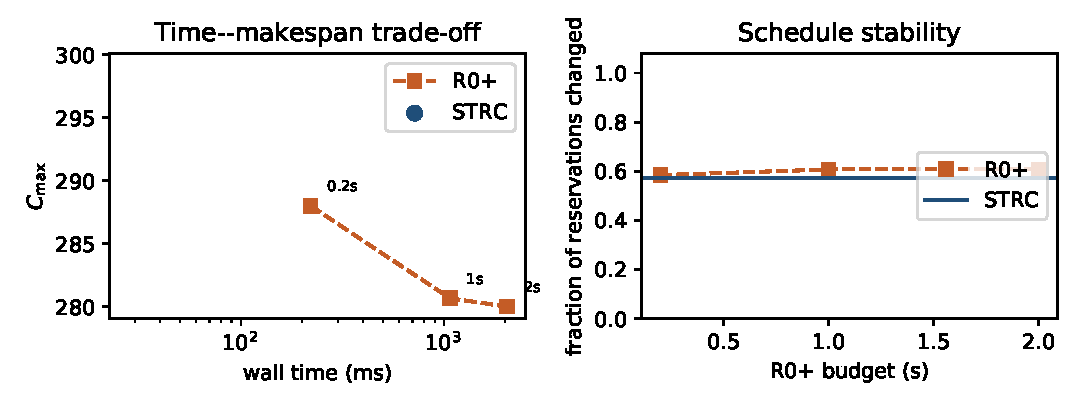
\includegraphics[width=\linewidth]{figures/fig_strc_e5}
\caption{E5: budget sweep of R0+ (which does not rewrite finished occupancies) versus bounded repair (\texttt{congested\_8x4x4}, mean over \(3\) random seeds).
Left: runtime versus \(C_{\max}\); the two curves do not intersect. Right: occupancy rewrite fraction, about \(0.6\) for both methods.}
\Description{Two side-by-side plots. The left plot has runtime on a logarithmic horizontal axis and makespan on the vertical axis:
warm-started global rescheduling that does not rewrite finished occupancies decreases slightly with the budget, while bounded repair is a single point at the upper left;
the two do not intersect, and global rescheduling is slightly lower at every budget point. The right plot shows the occupancy rewrite fraction,
about 0.6 for both methods.}
\label{fig:e5}
\end{figure}

Bounded repair yields a worse makespan over the entire budget range, but its runtime is two to three orders of magnitude lower (\(\MsRepairMed\)\,ms for level-1 rerouting
versus budgets of \(0.2\)--\(2\)\,s; see Figure~\ref{fig:e5}, left). This runtime gap comes from a single rerouting pass that does not restart the search;
it does \emph{not} come from scoping on the impact set, as Section~\ref{sec:cheap} confirms with the RA baseline of equal runtime.
The rewrite fractions of the two methods are of the same order, \ResFracRtwo; for a comparison of rewrite volume, see the RA comparison in Section~\ref{sec:cheap}.
When a millisecond-scale response is required, bounded repair restores feasibility; when a stoppage of seconds is acceptable, warm-started global rescheduling that does not rewrite finished occupancies achieves a better makespan.

The R0+ in this table uses the fixed-prefix decoding of Section~\ref{sec:vs_r0} and does not rewrite finished occupancies.
A check for rewrites of finished occupancies found \(\RzeroPastLo\) violations at each of the \(9\) budget points of both the small and the congested instance.
When a later operation of a job has already been carried away by a vehicle while an earlier operation still needs retiming, R0+ keeps the original vehicle and replans only the tail after \(t_{\mathrm{now}}\),
thereby preserving the already executed empty-leg prefix. Bounded repair likewise has zero violations in the same cells.
The makespan gap between the two therefore contains no contribution from ``rewriting finished occupancies'';
the remaining gap comes from the advantage of global reassignment and resequencing over a single rerouting pass.
Consequently, the value of the reservation impact set does not lie in the makespan; its intended use is recovery that must respond within milliseconds.

%% No \(\times\) in the title: it goes into the PDF bookmarks, and hyperref cannot handle math mode there.
\subsection{E6: crossing disturbance types with scope objects}
\label{sec:e6}

E1--E3 consider only one disturbance, corridor blockage. This subsection expands the disturbance-type dimension: on the same \(\NPairs\) pairs we add
three further types, namely corridor slowdown, vehicle failure, and robotic-arm failure. The results are given in Table~\ref{tab:e6}.

\textbf{What is measured.} For scoping, we report for all four disturbance types the size of the affected set on the operation-precedence graph, the size of the reservation impact set, and whether the latter contains the former.
For repair, we run the repair for all four types. Class B still uses rerouting only: a blockage writes the no-entry window into the reservation table, while a slowdown reduces traversal progress by a factor of
\(\tau_{\mathrm{mult}}=2\) within the window, traversal outside the window follows the original \(\tau\), and the corridor remains passable.
Class A additionally allows vehicle swapping or machine reassignment, without changing the processing order; whether the rewritable scope is escalated does not affect its action set.

\begin{table}[t]
\centering
\caption{E6 disturbance type \(\times\) scope object (\(\NPairs\) pairs per type, \(200\) measurements in total;
the two Class B disturbances produce the same seed set by construction, so there are \(150\) \emph{independent} scoping measurements; see the third point in the text).
\(|R^{\circ}|\) is the number of occupancies unfinished after \(t_{\mathrm{now}}\).
``R1 empty'' is the number of cells in which scoping on the operation-precedence graph deems the disturbance to require no rescheduling.
The last column uses no scope escalation: level-1 rerouting for Class B, and vehicle swapping or machine reassignment for Class A.}
\label{tab:e6}
\small
\begin{tabular}{@{}llccccc@{}}
\toprule
Disturbance & Class & R1 empty & Mean \(|U_{R1}|\) & Mean \(|\mathrm{Cl}|\)
 & \(\mathrm{Cl}/|R^{\circ}|\) & R2 feasible \\
\midrule
Corridor blockage   & B & \(50/50\) & \(0.0\)  & \(64.4\) & \(0.92\) & \FeasESixBlock \\
Corridor slowdown & B & \(50/50\) & \(0.0\)  & \(64.4\) & \(0.92\) & \FeasSlow \\
Vehicle failure   & A & \(0/50\)  & \(31.1\) & \(60.6\) & \(0.85\) & \FeasESixAgv \\
Robotic-arm failure & A & \(0/50\)  & \(42.8\) & \(65.9\) & \(0.94\) & \FeasESixRa \\
\bottomrule
\end{tabular}
\end{table}

The results comprise four points. First, \textbf{the A/B dichotomy holds without exception over the \(150\) \emph{independent} scoping measurements} (the two Class B disturbances share the same seed set; see the third point): scoping on the operation-precedence graph
is empty for both Class B disturbances in every case and nonempty for both Class A disturbances in every case. Second, \textbf{over all \(100\) Class A measurements,
\(U_{R1}\subseteq\mathrm{Cl}\)}; that is, on Class A, switching to scoping on the reservation impact set never \emph{misses}
an occupancy already included by the operation-precedence graph. The containment is strict in \(\StrictlyLarger\) cells, and the two sets are equal in the remaining \(13\) cells.
For the robotic-arm failure row, containment holds \emph{by construction}: the seed rule of Definition~\ref{def:seeds}(c) takes the entire suffix along the job chain,
whereas \(U_{R1}\) is truncated at \(\theta=2\) (Section~\ref{sec:protocol}); this row thus only verifies that the implementation agrees with the definition.
For the vehicle failure row, containment is an empirical result.
The price is a larger rewritable set on average: \(31.1\to 60.6\) for vehicle failure and \(42.8\to 65.9\) for robotic-arm failure.
Third, \textbf{slowdown and blockage produce identical scoping results cell by cell}, with the same impact-set size on all \(50\) pairs.
The reason is that the two share the same seed rule (unfinished occupancies overlapping the failure window), which by construction yields the same reservation impact set;
the row shows that scoping on the operation-precedence graph also yields an empty scope for slowdown.
Fourth, \textbf{for repair, all four disturbance types are feasible in every case}; per-type results are in the last column of Table~\ref{tab:e6}, with slowdown measured on the same basis as blockage.
A slowdown only scales the progress of the part overlapping the window, and the corridor remains passable,
so it still differs physically from ``full no-entry followed by a detour''. Level-1 rerouting already achieves full feasibility, and scope escalation is never triggered.
Vehicle failure is handled by vehicle swapping and robotic-arm failure by machine reassignment.

\textbf{This table also provides an empirical measure of the impact-set size} (Remark~\ref{rem:minimality}).
Under corridor blockage, the reservation impact set covers about \(\ClosureAliveFrac\) of the occupancies unfinished after \(t_{\mathrm{now}}\);
compared with the trivial upper bound of ``including all unfinished occupancies in the rewrite'', it includes less than one tenth fewer.
This does not contradict the range \EoneCloLo--\EoneCloHi\ of \(\mathrm{Cl}/|R|\) computed over the whole table in Section~\ref{sec:e1}:
the whole table also contains the roughly half of the occupancies that were completed before \(t_{\mathrm{now}}\) and cannot be rewritten.
In terms of contributions, this subsection extends the conclusions of C1 and C2 from one disturbance type to four.

\subsection{E7: comparisons within the millisecond range}
\label{sec:cheap}

The baseline in E5 is a warm-started population search with a budget of \(0.2\)--\(2\)\,s. Using it as the only baseline leaves a question open:
\emph{how much of the ``two to three orders of magnitude lower'' result is due to the reservation impact set, and how much merely to the longer runtime of the baseline?}
This subsection adds baselines whose runtime lies between those of bounded repair and warm-started population search, together with a baseline that changes only the rewritable scope.

\begin{itemize}[leftmargin=1.5em,itemsep=0.25em]
\item \textbf{RS (global right shift).} Without changing routes, assignments, or processing orders, RS postpones all unfinished occupancies as a whole
by a delay \(\Delta\), where \(\Delta\) is just large enough to move every movable occupancy on the blocked corridor past the blockage window.
Like R2, it does not rewrite finished occupancies (those with \(t^e\le t_{\mathrm{now}}\) are immovable).
Because the shift is uniform, every time gap stays the same or grows, and all constraints are of the ``\(\ge\)'' type,
so a feasible solution is obtained without rerouting. RS represents one extreme of ``\emph{not scoping on the impact set}'' and performs no rerouting at all
(Section~\ref{sec:rw_aor}).
\item \textbf{RD (re-decoding of the original chromosome).} RD keeps the machine assignments and processing orders and runs the same fixed-prefix decoding as R0+
on the routing layer into which the blockage has been written. It is the \emph{fastest global recomputation} in our implementation; because it does not change the chromosome, it is faster than R0+
but has less freedom to reassign and resequence.
\item \textbf{RA (no scope restriction by the impact set, but with rerouting retained).} RA includes all occupancies \emph{unfinished} after \(t_{\mathrm{now}}\) in the rewrite
and then runs a rerouting replay \emph{identical} to that of R2. It represents the other extreme of ``not scoping on the impact set'': unlike RS, it retains
rerouting, so its only difference from R2 is the set of rewritable occupancies. The two use the same rerouting procedure, neither rewrites finished occupancies, and both face the same blockage.
RA is therefore the \emph{only} baseline in this paper that isolates the effect of the reservation impact set; the difference between the two methods contains no contribution from the rerouting procedure, the protocol, or the implementation.
Since RA's rewritable set is already maximal, it needs no scope escalation after failure.
\end{itemize}

E3 compares two \emph{different} scope objects (the operation-precedence graph and the reservation impact set), whereas RA addresses the question
\emph{whether the rewritable scope needs to be restricted by the impact set at all}.

\begin{table}[t]
\centering
\caption{E7 comparisons within the millisecond range (\(\NPairs\) pairs; same protocol as E3: single-window blockage of a busy corridor,
\(t_{\mathrm{now}}=0.35\,C_{\max}^{0}\), R2 without scope escalation). All four methods are feasible in \(\NPairs/\NPairs\) cases.
``Finished-occupancy violations'' is the number of cells in which finished occupancies were rewritten; ``Rewritable'' is the share of occupancies unfinished after \(t_{\mathrm{now}}\)
that the method includes in the rewrite; the last column gives the method's \(C_{\max}\) win/tie/loss against R2. RA and R2 differ only in which occupancies are rewritable,
so the entire difference between these two rows is attributable to the reservation impact set. This table is \emph{not} directly comparable with Table~\ref{tab:e5}, which contains only two instances.}
\label{tab:cheap}
\small
\begin{tabular}{@{}lcccccc@{}}
\toprule
Method & \makecell{Finished-occupancy\\violations} & \makecell{ms\\(median)} & \makecell{Mean\\degradation} & \makecell{Rewrite\\fraction} & Rewritable & \makecell{W/T/L\\vs.\ R2} \\
\midrule
RS global right shift      & \ShiftBad     & \MsShift    & \(58.8\%\) & \ResFracShift    & ---   & \(7/16/27\) \\
RD re-decoding        & \RedecodeBad  & \MsRedecode & \(49.0\%\) & \ResFracRedecode & ---   & \(22/14/14\) \\
RA no impact-set scoping & \ShiftBad     & \MsAllFuture & \(49.9\%\) & \ResFracAllFuture & \(1.00\) & \(0/46/4\) \\
R2 bounded repair      & \ShiftBad     & \MsCheapRtwo & \(49.8\%\) & \ResFracCheapRtwo & \ClosureShareMean & --- \\
\bottomrule
\end{tabular}
\end{table}

Table~\ref{tab:cheap} yields four findings.

\textbf{First, among the methods that return a feasible plan, the only one faster than bounded repair is the global right shift,
but it is worse in both makespan and rewrite fraction.} (R1, which scopes on the operation-precedence graph, is faster, but its feasibility rate is only \FeasRone,
so it is not a candidate method.)
RS needs only \MsShift\,ms, about half the time of R2. The price is a mean makespan degradation of \(58.8\%\) (versus
\(49.8\%\) for R2), a cell-by-cell result of \WinVsShift\ (R2 win/tie/loss), and more rewritten occupancies
(\ResFracShift\ vs.\ \ResFracCheapRtwo), because the uniform shift changes the times of every unfinished occupancy.
Making the right shift \emph{selective}, that is, delaying only the vehicles actually affected and leaving the rest unchanged, would first require
determining which occupancies are affected, which is precisely the scope this paper delineates. \textbf{The right shift needs no impact-set scoping precisely because
it gives up selectivity.}

\textbf{Second, even the fastest global recomputation is slower than bounded repair.} The median runtime of RD is
\MsRedecode\,ms, \RedecodeRatio\ times that of R2. This result does not depend on the search configuration: any decoding-based search
needs at least one decoding per candidate evaluated. The ``two to three orders of magnitude lower'' result in E5 is therefore \emph{not}
an artifact of an overly slow baseline; with the baseline replaced by the fastest global recomputation in the same implementation, bounded repair is still faster.

\textbf{Third, without rewriting finished occupancies, RD and R2 are indistinguishable in makespan on this sample, but RD rewrites more.}
Over the whole table, R2 versus RD is \WinVsRedecode\ (win/tie/loss), with mean degradations of \(49.8\%\) and \(49.0\%\). The difference is not significant:
the mean paired difference is \(+0.006\) with a bootstrap \(95\%\) interval of \([-0.007,\,0.019]\), which contains \(0\); the two-sided Wilcoxon signed-rank test
gives \(p=0.12\) (\(36\) cells with nonzero differences); and the mean \(C_{\max}\) ratio is \(0.997\) with interval \([0.988,\,1.007]\), which likewise contains \(1\).
No makespan difference between the two is thus observed.
RD has \RedecodeBad\ finished-occupancy violations: when a later operation has already been carried away by a vehicle, RD keeps the original vehicle and replans only the tail after the decision time,
thereby preserving the already executed empty-leg prefix. RD's slight edge in the cell-by-cell count therefore stems from the advantage of global rerouting under the same chromosome over a single rerouting pass,
not from rewriting finished occupancies. RD's rewrite fraction is \ResFracRedecode, higher than R2's
\ResFracCheapRtwo; that is, the method that scopes on the impact set rewrites less.

\textbf{Fourth, the reduction in rewrite volume can be established only by comparing R2 with RA, and it manifests only as stability.} RA and R2 differ only in the set of rewritable occupancies, so this pair
directly gives the net benefit of scoping on the impact set. On average, the reservation impact set includes only \(1-\ClosureShareMean\) fewer
unfinished occupancies than the trivial upper bound (\ClosureShareLo--\(1.00\) per cell; in the \(6\) cells with value \(1.00\), the impact set \emph{equals}
the set of all unfinished occupancies, and the two methods give identical results). This difference of less than one tenth lowers the rewrite fraction from \ResFracAllFuture\ to
\ResFracCheapRtwo: a mean reduction of \RAStabMean, a median reduction of \RAStabMed, a cell-by-cell result of \RAStabWTL\ (R2 more stable/tie/less stable),
and a two-sided Wilcoxon signed-rank \(p=\RAStabP\).

Excluding the \(6\) identical cells above leaves \(44\) cells, with a cell-by-cell result of \RAStabWTLNet\ and a mean reduction of \RAStabMeanNet\
(the Wilcoxon test has \(32\) cells with nonzero differences under both counts); the reduction reported over \NPairs\ cells is thus conservative.
The direction of the reduction is highly consistent, but its \emph{magnitude is small}; in the single counterexample cell, R2 rewrote \(0.007\) more.
Meanwhile, the two methods have nearly identical runtimes (\MsCheapRtwo\ vs.\ \MsAllFuture\,ms)
and nearly identical makespans (mean ratio \RACmaxRatio; cell-by-cell R2 win/tie/loss of \WinVsAllFuture, never worse,
with \RACmaxLo\ in the best cell).

These three results must be read together. \textbf{Equal runtime shows that the millisecond-scale response comes from a single rerouting pass that does not restart the search, not from the reservation impact set
(results in Table~\ref{tab:cheap}; single-pass rerouting itself is an existing technique, see Table~\ref{tab:position}).
Equal makespan shows that the impact set is not an optimization device.
A significantly lower rewrite fraction shows that scoping delivers exactly the property guaranteed by Proposition~\ref{prop:outside}: occupancies outside the set keep their corridors, intervals, and vehicles unchanged.}
The role of the impact set is to \emph{mark which occupancies need not be rewritten}.
The more occupancies the impact set excludes, the larger the reduction; however, the excluded occupancies themselves account for only part of
the gap \(\ResFracAllFuture-\ResFracCheapRtwo\); the rest comes from changes in the rerouting outcome once the rewritable set shrinks.
On the instance where the impact set nearly equals the set of all unfinished occupancies (\texttt{congested\_8x4x4}, rewritable share \(0.94\)),
the reduction is only \(0.010\); on the instance that excludes more occupancies (\texttt{S8x4x4\_mid}, \(0.91\)), the reduction reaches \(0.118\).
% selfcheck:allow-num 0.91 is this instance's rewritable share; it coincides in value with \ScaleCloAliveHi (upper bound of E8 level means) but comes from a different source
Two instances can only indicate a direction; the per-cell distribution is given below.

We next condense this direction into a post hoc threshold rule. Figure~\ref{fig:worth} plots the \(\NPairs\) pairs with the rewritable share
\(\mathrm{Cl}/|R^{\circ}|\) on the horizontal axis and the reduction in rewrite fraction of R2 relative to RA on the vertical axis.
On this sample we take \(\mathrm{Cl}/|R^{\circ}|\ge\WorthThresh\): the \WorthHighN\ cells above this line have a mean reduction of
\WorthHighMean, and the \WorthLowN\ cells below it have a mean reduction of \WorthLowMean.
All cells with a share above \(\WorthVanish\) show zero reduction, but for two different reasons. In the \(6\) cells whose share is exactly \(1.00\),
the impact set equals the set of all unfinished occupancies, so the two methods are \emph{identical}; in the remaining cells, the share is below \(1.00\) yet the reduction is already \(0\),
which is an empirical result rather than an identity.
The threshold is chosen on this sample to answer ``when does scoping on the impact set still pay off''; it is not meant to be extrapolated,
and it differs from a structural prediction of the impact-set size (Section~\ref{sec:e4}).

\begin{figure}[t]
\centering
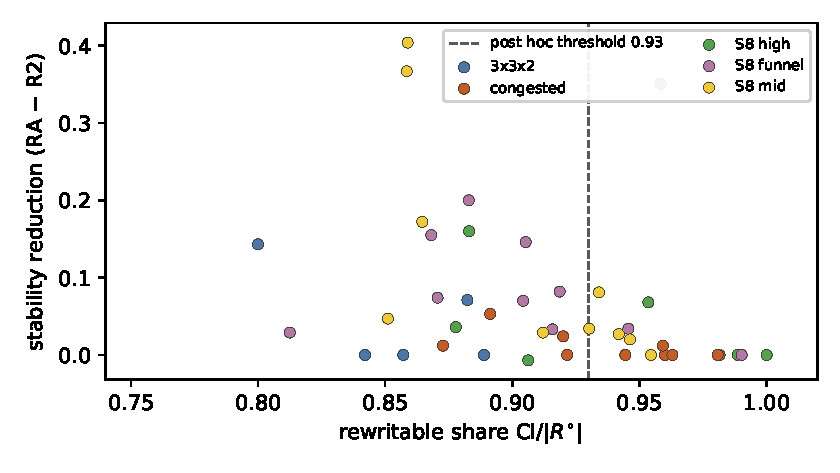
\includegraphics[width=0.92\linewidth]{figures/fig_strc_worth}
\caption{E7 post hoc rule: rewritable share versus reduction in rewrite fraction (\(\NPairs\) pairs, R2 vs.\ RA).
The dashed line marks the in-sample threshold \(\WorthThresh\); positive values on the vertical axis mean a lower rewrite fraction with impact-set scoping.}
\Description{Scatter plot. The horizontal axis is the share of unfinished occupancies covered by the reservation impact set, and the vertical axis is the additional share of occupancies rewritten without impact-set scoping relative to with it.
The five instances are distinguished by color, and a vertical dashed line is drawn at \WorthThresh. The points run roughly from upper left to lower right.}
\label{fig:worth}
\end{figure}

Combining the results of the four methods: under the two constraints that ``finished occupancies are not rewritten'' and that ``the response must be within milliseconds'',
\textbf{the net benefit of scoping on the impact set appears only in the rewrite volume.}
\textbf{At equal speed and makespan, forgoing scoping rewrites about \(6\) percentage points more occupancies (a relative increase of about \(12\%\))},
whereas scoping brings \emph{no} advantage in speed or makespan.
When the runtime constraint is relaxed, a shorter makespan still comes from warm-started search (Section~\ref{sec:e5}),
but its runtime then exceeds the millisecond range.

